%In today's world, artificial intelligence has proved to be a game-changer in designing agents that interact with an evolving environment and make decisions on the fly. The main goal of artificial intelligence is to design artificial agents that make dynamic decisions in an evolving environment. In pursuit of these, the agent can be thought of as making a series of sequential decisions by interacting with the dynamic environment which provides it with some sort of feedback after every decision which the agent incorporates into its decision-making strategy to formulate the next decision to be made. A large number of problems in science and engineering, robotics and game playing, resource management, financial portfolio management, medical treatment design, ad placement, website optimization and packet routing can be modeled as sequential decision-making under uncertainty. Many of these real-world interesting online 
%sequential decision-making problems can be formulated as reinforcement learning (RL) problems (\citep{bertsekas1996neuro}, \citep{sutton1998reinforcement}). 


In today's world, artificial intelligence has proved to be a game-changer in designing agents that interact with an evolving environment and make decisions on the fly. The main goal of artificial intelligence is to design artificial agents that make dynamic decisions in an evolving environment. In pursuit of these, the agent can be thought of as making a series of sequential decisions by interacting with the dynamic environment which provides it with some sort of feedback or reward after every decision which the agent incorporates into its decision-making strategy to formulate the next decision to be made. In its simplest form, this problem can be captured by the multi-armed bandit (MAB) model \citep{bertsekas1996neuro}, \citep{sutton1998reinforcement}. 

	The name bandit originated from the concept of casino slot machine where there are levers which are termed as arms and the learner can pull one arm and observe the reward associated with that arm. This reward is sampled from a probability  distribution associated with that specific arm and is considered as the feedback revealed by the environment. This game is repeated $T$ times and the goal of the learner is to maximize its profit by finding an action-selection strategy or policy that optimizes some long-term performance measure. 
	
	%Infact the MAB model can be considered as a single looping state when the agent after taking an action, and observing the reward transitions back to the same state. That single looping state consist of several finite number of actions which are called as arms.


	There are multiple reasons to study the interesting area of bandits. First of all, bandits are the cornerstone of understanding the general reinforcement learning area. Infact, bandits helps us to understand the idea of \textit{exploration-exploitation} dilemma which forms the foundation to build full, multi-state, general reinforcement learning models. Secondly, as stated in \citet{maillard2011apprentissage}, even $50$ years after \cite{robbins1952some} introduced the first idea of bandits, there are many interesting and fruitful areas where bandit concept can be extended in both practical and theoretical terms. Finally, there are several real-life industrial applications ranging from recommendation systems, game theory to anomaly detection where bandit applications have been found to perform exceptionally well. All of these forces us to delve deep into a systemic research of bandits.

	
%In an RL problem, an agent interacts with a dynamic, stochastic, and unknown environment, with the goal of finding an action-selection strategy or policy that optimizes some long-term performance measure. Every time when the agent interacts with the environment it receives a signal/reward from the environment based on which it modifies its policy. The agent learns to optimize the choice of actions over several time steps which is learned from the sequences of data that it receives from the environment. This is the crux of online sequential learning. 
%
%    This is in contrast to supervised learning methods that deal with labeled data which are independently and identically distributed (i.i.d.) samples from the considered domain and train some classifier on the entire training dataset to learn the pattern of this distribution to predict the labels of future samples (test dataset) with the assumption that it is sampled from the same domain. In contrast to this, an RL agent learns from the samples that are collected from the trajectories generated by its sequential interaction with the system. For an RL agent, the trajectory consists of a series of sequential interactions whereby it transitions from one state to another following some dynamics intrinsic to the environment while collecting the reward till some stopping condition is reached. This is known as an episode. Here, for an action $i_t$ taken by the agent at the $t$-th timestep, the agent transitions from its current state denoted by $S_{i,t}$ to state $S_{i,t+1}$ and observes the reward $X_{i,t}$. An illustrative image depicting the reinforcement learning scenario is shown in Figure \ref{fig:rl}.
%
%\begin{figure}[!th]
%\begin{center}
%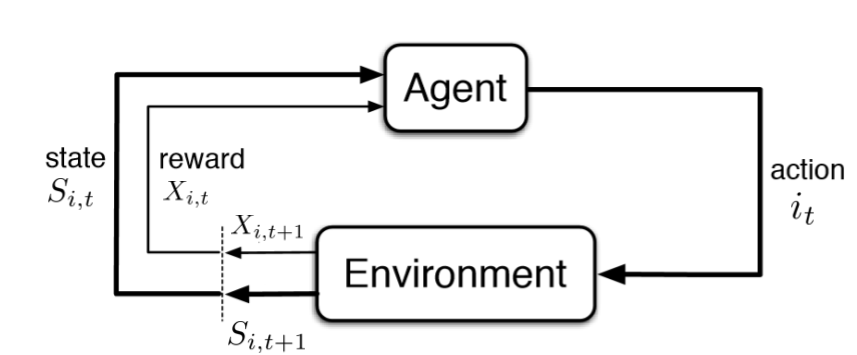
\includegraphics[scale=0.3]{synopsis/img/RL1.png}
%\caption{Reinforcement Learning}
%\label{fig:rl}
%\end{center}
%\end{figure}

%Now, for a single-step interaction, i.e., when the episode terminates after a single transition, the problem is captured by the multi-armed bandit (MAB) model. Infact the MAB model can be considered as a single looping state when the agent after taking an action, and observing the reward transitions back to the same state. That single looping state consist of several finite number of actions which are called as arms.

%	The name bandit originated from the concept of casino slot machine where there are levers which are termed as arms and the learner can pull one lever and observe the reward associated with that arm which is sampled from a distribution associated with the specific arm. This game is repeated $T$ times and the goal of the learner is to maximize its profit. 
	
	
    
    
%To express an RL problem more formally, we have to define the idea of Markov Decision Process (MDP) which consists of states, actions, transition probabilities, and rewards which in turn helps in deciding the strategy to be followed by the agent. 

%An MDP consists of states
